\section{Graphen und Netzwerke}
\begin{tabularx}{\textwidth}{p{4cm} X}
  Exakter Algorithmus
    & Findet optimale Lösung\\
  Heuristik
    & Findet gute, aber normalerweise nicht optimale Lösung\\
  Greedy Algorithmus
    & Trifft zu jedem Zeitpunkt aktuell beste Wahl, d.h. lokales Optimum; müssen nicht zu globalen Optimum führen \\
  Ungerichteter Graph
    & Graph mit endlicher Menge Ecken $V$ und Kanten $v,w \in E$\\
  Einfacher Graph
    & Keine Schlingen, keine parallelen Kanten \\
  Schlinge
    & Kante, wo Anfang- gleich Endecke ist ($vv$)\\
  Pfad 
    & Folge von Ecken $v_0, v_1, ... v_k$\\
  Kreis 
    & Pfad, wo die Anfangsecke gleich der Endecke: $v_0 = v_k$\\
  Azyklischer Graph, Wald
    & Graph, der keinen Kreis enthält\\
  Baum
    & Azyklischer, zusammenhängender Graph\\
  Bipartiter Graph
    & Die Ecken können in zwei Teilmengen aufgeteilt werden, so dass jede Kante je eine Ecke in beiden Teilmengen hat \skript{10}\\
  Eulerkreis
    & Kreis, der jede Kante des Graphen genau ein Mal enthält\\
  Hamiltonkreis
    & Kreis, der alle Ecken genau ein Mal besucht und zudem in der Startecke endet\\
  Euler-/Hamiltongraph
    & Wenn Graph einen Euler- oder Hamiltonkreis enthält\\
\end{tabularx}


\subsection{Repräsentation von Graphen \skript{3}}
  Adjazenzmatrix, Adjazenzliste
  
\subsection{Entscheidungsbaum-Verfahren \skript{4}}
	Das Travelling-Salesman-Problem (\skript{31}), wo jede Stadt genau ein Mal besucht werden darf, ist lösbar mit dem Branch-And-Bound Verfahren.
	
\subsection{Traversieren von Graphen \skript{9}}
	\subsubsection{Tiefensuche (Depth-First Search, DFS)}
		Ausgehend von einer Ecke, wird immer weiter zur nächsten Ecke durch den Baum "traversiert", bis das Ende erreicht ist. Dann wird von der nächsten unbesuchten Ecke weitertraversiert, bis alle Ecken besucht sind. Dies ist eine Last-In-First-Out (LIFO) Strategie.
	
	\subsubsection{Breitensuche (Breadth-First Search, BFS)}
  	Von einer Ecke werden alle benachbarten Ecken aufgesucht und im nächsten Schritt einer dieser benachbarten Ecken besucht. Dies ist eine First-In-First-Out (FIFO) Strategie.
	
\subsection{Aufspannende Bäume \skript{11}}
	MST = Minimal aufspannender Baum: Summe aller Kantengewichte ist minimal unter allen verbundenen Knoten.
	
	\begin{tabularx}{\textwidth}{p{4cm} X p{4cm}}
	  \textbf{Prim}-Algorithmus
	    & Läuft über Ecken
	    & $O(n^2)$ \\
	  \textbf{Kruskal}-Algorithmus
	    & Läuft über Kanten
	    & $O(m \log(m))$\\
	  MST-Heuristik
	    & Von bestehendem MST aus, wird in beliebige Richtung iteriert
	    & $O(n)$ ??
	\end{tabularx}

\subsection{Minimale Wege \skript{13}}
  \subsubsection{Probleme}
    \begin{tabular}{ll}
      Source-sink shortest path
        & Kürzesten Weg zwischen Quelle/source und Senke/sink \\
      Single source shortest paths
        & Kürzeste Wege zwischen einer Quelle/source zu allen anderen Ecken \\
      All pairs shortest paths
        & Kürzeste Wege zwischen allen Eckenpaaren\\
    \end{tabular}
  \subsubsection{Algorithmen}
    \begin{tabularx}{\textwidth}{p{3cm} p{4cm} X r}
      \textbf{Algorithmus} & \textbf{Löst} & \textbf{Bemerkungen} \\
      \textbf{Dijkstra} 
        & Source-sink shortest path, single source shortest path
        & Kantengewichte $\geq$ 0; Greedy; Loop über alle bereits besuchten Ecken: Suche minimale Distanz zu nächster Ecke, der Weg, der am Schnellsten am Ziel ist, gewinnt.
        & $O(n^2)$\\
      \textbf{Bellman-Ford}
        & Source-sink shortest path, single source shortest path
        & Auch negative Kantengewichte möglich 
        & ?\\
      \textbf{A*} 
        & Single source shortest path
        & Heuristische Methode, beschleunigte Laufzeit
        & ?\\
      \textbf{Floyd-Warshall }
        & All pairs shortest paths 
        &
        & $O(2n^3)$\\
    \end{tabularx}
	
\subsection{Flüsse in Netzwerken \skript{18}}
  Jede Kante $vw$ hat jetzt auch eine Kapazität $c(vw)$, welche eine Obergrenze für den Fluss $f(vw)$ darstellt. Zusätzlich können den Kanten noch Kosten $k(vw)$ angefügt werden.
  
  \begin{tabularx}{\textwidth}{l X}
    Verteilungsproblem
      & Objekte von einem oder mehreren Orten (sources) an eines oder mehrere Ziele (sinks) zu verteilen\\
    Matching-Probleme
      & Zuordnung von Mengen, kann auch als bipartite Graphen interpretiert werden (bspw. Partnervermittlung) \\
    Schnitt-Probleme
      & Kanten entferne, um Netzwerk zu zerlegen (bspw. max. Anzahl Unterbrüche in Kommunikationsnetz)\\
  \end{tabularx}
  
\subsection{Maximale Flüsse \skript{20}}
  \begin{minipage}{13.7cm}
    Gesucht wird der maximal mögliche Fluss zwischen einer Quelle $s$ zu einer Senke $t$ ($st$-Netzwerk). Ermittlung mit \textbf{Ford-Fulkerson}-Algorithmus, der auch Rückwärtsflüsse beachtet.
    
    Das \textbf{Max-Flow Min-Cut} Theorem besagt, dass der maximale Fluss in einem $st$-Netzwerk gleich dem minimalen Fluss über alle möglichen $st$-Schnitte ist.
  \end{minipage}
  \begin{minipage}{5cm}
    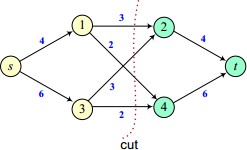
\includegraphics[width=5cm]{./Content/GraphsAndNetworks/max-flow-min-cut}
  \end{minipage}

\subsection{Reduktionen auf Maxflow-Probleme \skript{25}}
  \begin{minipage}{9.5cm}
    \begin{liste}
      \item Mehrere Quellen können zu einer Quelle zusammengefasst werden, ebenfalls bei Senken (Bild rechts)
      \item Maximalwerte pro Ecke können mit zusätzliche Ecken hinzugefügt werden.
      \item Weitere Ideen...
    \end{liste}
  \end{minipage}
  \begin{minipage}{9.5cm}
    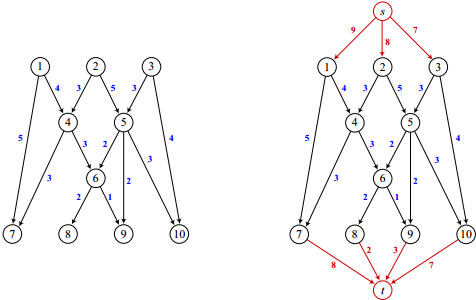
\includegraphics[width=9.5cm]{./Content/GraphsAndNetworks/maxflow-reduktion}
  \end{minipage}